\section{Bayesian Network}
\label{sec:bayesiannet}
Bayesian Networks allow us to \textbf{economically encode a probability distribution} over a set of variables, stating the \textbf{conditional independencies} across the different variables, a rather interesting notion in the analysis of this problem. They are a sufficient and compact specification of the full joint distribution. No Bayesian Network of the problem was available, but luckily the Python library \texttt{pgmpy} has exactly what is needed for us to obtain the network and its \textit{Conditional Probability Tables} from the dataset.
\subsection{Structure learning}
To learn the model structure, i.e. a Directed Acyclic Graph, there are \textbf{two different families of techniques} that can be chosen: the constraint-based approaches, which search for a graph structure satisfying the independence assumptions that we observe in the empirical distribution; and the score-based approaches, which define an objective function for different models, and then search for a high-scoring model. \cite{book:probgraphmod}
The approach I chose is the latter, needing a \textbf{scoring function} $s_D: M \rightarrow \mathbb{R}$, which maps a model $x \in M$ to a real score, based on how well it fits to the given dataset. Then, a search strategy traverses the space of all possible models and selects the one with optimal score. Several scoring functions are available, such as \textit{BDeu}, \textit{K2} and \textit{BIC}. The last one, \textit{Bayesian Information Criterion}, is a good asymptotic approximation of the likelihood of the training data. After having defined a scoring function, we can choose different search strategies, usually \textit{local searches}, i.e. iterative search algorithms that keep improving a solution until a local maxima is reached. The algorithm I chose is \textbf{Hill Climb Search}, a rather simple algorithm that is able to explore the search space (while still not being extraordinarily performant) and find a good solution. 
To learn the network structure through \texttt{pgmpy}, we'll first have to import the data in a Pandas DataFrame:
\begin{minted}{python}
import pgmpy
import pandas as pd
cars_data = pd.read_csv('data/car.data', names=["Buying", "Maintenance",
"Doors", "People", "LugBoot", "Safety", "Acceptability"])
\end{minted}
Then, we'll just use \textit{pgmpy}'s \texttt{HillClimbSearch} with a \texttt{BicScore}:
\begin{minted}{python}
from pgmpy.estimators import HillClimbSearch
from pgmpy.estimators import BicScore

hc = HillClimbSearch(cars_data, scoring_method=BicScore(cars_data))
best_model = hc.estimate()
\end{minted}

\subsubsection{Learned graph}
After some instants, the search finds its best guess of model. We can therefore print its \textbf{edges} with \texttt{best\_model.edges()} obtaining the following result:
\begin{center}
\texttt{[('Buying', 'Maintenance'), ('Safety', 'People'), ('Safety', 'LugBoot'), ('Acceptability', 'Safety'), ('Acceptability', 'People'), ('Acceptability', 'Buying'), ('Acceptability', 'Maintenance'), ('Acceptability', 'LugBoot')]}
\end{center}
which, in a more graphically appealing way, is the following graph:
\begin{figure}[ht]
    \centering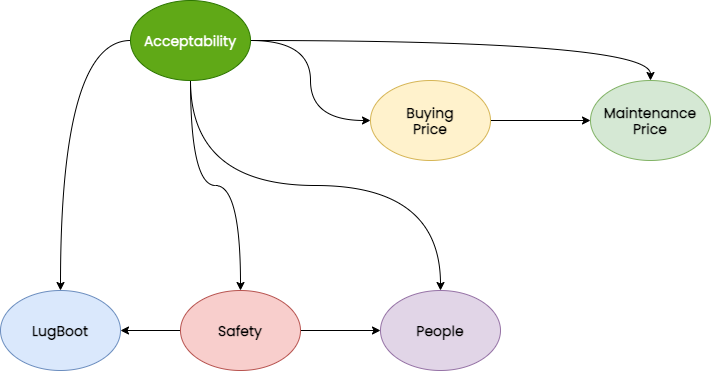
\includegraphics[width=0.8\linewidth]{figures/DAG.png}
    \caption{Bayesian network for the cars dataset}
    \label{fig:errors}
\end{figure}

\subsection{Parameter learning}
Now that we've found a good structure for our graph, we'll have to find the values of the Conditional Probability Distributions. The library \texttt{pgmpy} is a great tool for this task too. If one would have to find a solution for this problem, it would be pretty natural to think about the \textbf{relative frequencies} of the variable states. This approach is, basically, what \textit{Maximum Likelihood Estimation} does: as seen in section 17.1 of \cite{book:probgraphmod}, the likelihood function for a given choice of parameters $\theta$ is the probability the model assigns the training data:
\begin{equation}
L(\boldsymbol{\theta}: \mathcal{D})=\prod_{m} P(\xi[m]: \boldsymbol{\theta})
\end{equation}
In other words, we want to maximize the probability $P(data|model)$. This, in practice, is done by computing the state counts and dividing by the conditional sample size.
MLE has a high possibility of overfitting on small very datasets. This, fortunately, is not our case, and we would otherwise have needed a different estimator, like Bayesian Parameter Estimation. We can estimate the parameters and print the CPDs with:
\begin{minted}{python}
from pgmpy.models import BayesianModel
from pgmpy.estimators import MaximumLikelihoodEstimator

bayesian_model = BayesianModel(best_model.edges())
bayesian_model.fit(cars_data, estimator=MaximumLikelihoodEstimator)
for cpd in bayesian_model.get_cpds():
    print(cpd)
\end{minted}
Having finally built our full joint distribution, we can proceed and \textbf{answer some questions through inference}.